\documentclass[border=0.8ex,svgnames,tikz]{standalone}
\usepackage{amsmath,mathtools}
\usepackage{fontspec}
\setmainfont{Source Serif 4}
\setsansfont{Source Sans 3}
\setmonofont{Source Code Pro}

\usetikzlibrary{positioning,chains}

\begin{document}
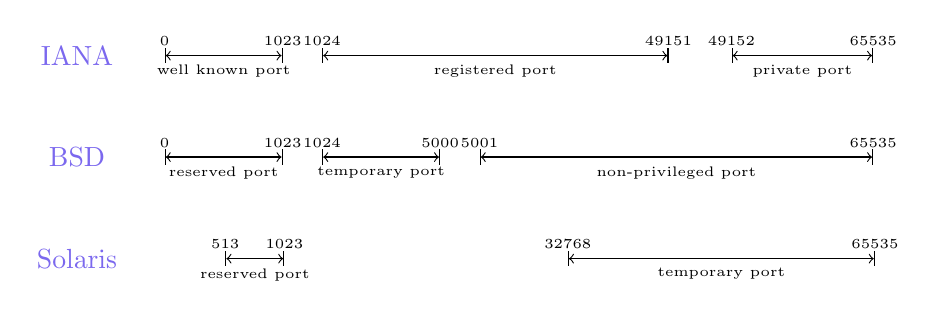
\begin{tikzpicture}
  \begin{scope}[
    every node/.style={
      on chain,
      text=MediumSlateBlue,
      minimum width=8ex,
    },
    start chain=going below,
    node distance=0.8,
    ]
    \node (iana)    {IANA};
    \node (bsd)     {BSD};
    \node (solaris) {Solaris};
  \end{scope}
  \begin{scope}[every path/.style={|<->|,draw},every node/.style={font=\tiny}]
    \coordinate[right=0.5 of iana] (inan-well-known-port-begin);
    \path(inan-well-known-port-begin) node[above]{0} -- node[below]{well known
      port} ++(1.5,0) coordinate(inan-well-known-port-end) node[above]{1023};
    \coordinate[right=0.5 of inan-well-known-port-end] (inan-registered-port-begin);
    \path (inan-registered-port-begin) node[above]{1024} -- node[below]{registered
      port} ++(4.4,0) coordinate(inan-registered-port-end) node[above]{49151};
    \coordinate[right=0.8 of inan-registered-port-end] (inan-private-port-begin);
    \path (inan-private-port-begin) node[above]{49152} -- node[below]{private port}
    ++(1.8,0) coordinate(inan-private-port-end) node[above]{65535};
  \end{scope}
  \begin{scope}[every path/.style={|<->|,draw},every node/.style={font=\tiny}]
    \coordinate[right=0.5 of bsd]  (bsd-reserved-port-begin);
    \path (bsd-reserved-port-begin) node[above]{0} -- node[below]{reserved port}
    ++(1.5,0) coordinate(bsd-reserved-port-end) node[above]{1023};
    \coordinate[right=0.5 of bsd-reserved-port-end] (bsd-temp-port-begin);
    \path (bsd-temp-port-begin) node[above]{1024} -- node[below]{temporary port}
    ++(1.5,0) coordinate(bsd-temp-port-end) node[above]{5000};
    \coordinate[right=0.5 of bsd-temp-port-end] (bsd-non-privileged-port-begin);
    \path (bsd-non-privileged-port-begin) node[above]{5001} --
    node[below]{non-privileged port} ++(5,0)
    coordinate(bsd-non-privileged-port-end) node[above]{65535};
  \end{scope}
  \begin{scope}[every path/.style={|<->|,draw},every node/.style={font=\tiny}]
    \coordinate[right=1.25 of solaris] (solaris-reserved-port-begin);
    \path (solaris-reserved-port-begin) node[above]{513} -- node[below]{reserved
      port} ++(0.75,0) coordinate(solaris-reserved-port-end) node[above]{1023};
    \coordinate[right=3.6 of solaris-reserved-port-end] (solaris-temp-port-begin);
    \path (solaris-temp-port-begin) node[above]{32768} -- node[below]{temporary
      port} ++(3.9,0) coordinate(solaris-temp-port-end) node[above]{65535};
  \end{scope}
\end{tikzpicture}
\end{document}
